\documentclass[12pt,a4paper]{report}
\usepackage{amsthm,amssymb,amsmath}
\usepackage[top=50mm, bottom=50mm, left=50mm, right=50mm]{geometry}

\usepackage{graphicx}
\usepackage{subcaption}
\usepackage[pagebackref=false,colorlinks,linkcolor=blue,citecolor=magenta]{hyperref}


\usepackage{geometry}
\usepackage{datetime} 
\usepackage{multirow}


\newcommand*{\BeginNoToc}{%
  \addtocontents{toc}{%
    \edef\protect\SavedTocDepth{\protect\the\protect\value{tocdepth}}%
  }%
  \addtocontents{toc}{%
    \protect\setcounter{tocdepth}{-10}%
  }%
}
\newcommand*{\EndNoToc}{%
  \addtocontents{toc}{%
    \protect\setcounter{tocdepth}{\protect\SavedTocDepth}%
  }%
}
\renewcommand{\bibname}{مراجع}
%\renewcommand{\refname}{مراجع}

%\usepackage[pagebackref=false]{hyperref}
\usepackage{tocbibind}
\usepackage{makeidx}
\makeindex
\usepackage{xepersian}
\settextfont[Scale=1.1]{B Nazanin}
% Latex 2020 2021 SetDigitFont error
\ExplSyntaxOn
\cs_set_eq:NN
\etex_iffontchar:D
\tex_iffontchar:D
\cs_undefine:N \c_one
\int_const:Nn \c_one { 1 }
\ExplSyntaxOff
\setdigitfont{Yas}
\defpersianfont\titr[Scale=1]{XB Titre}
\defpersianfont\nastaliq[Scale=1.5]{IranNastaliq}
\defpersianfont\traffic[Scale=1]{B Traffic}


\theoremstyle{definition}
\newtheorem{definition}{تعریف}[section]
\newtheorem{theorem}[definition]{قضیه}
\newtheorem{lemma}[definition]{لم}
\newtheorem{proposition}[definition]{گزاره}
\newtheorem{corollary}[definition]{نتیجه}
\newtheorem{remark}[definition]{ملاحظه}
\theoremstyle{definition}
\newtheorem{example}[definition]{مثال}


\begin{document}
	\newgeometry{total={210mm,297mm}, left=40mm, right=40mm, top=20mm, bottom=20mm,}
	\pagenumbering{harfi}
	\thispagestyle{empty}
	\vspace*{25mm}
	\centerline{
\includegraphics[height=4cm]{./images/logos/iust.png}}

	\begin{center}
	\textbf{
		دانشکده مهندسی کامپیوتر
	}
	\\[1cm]
	\baselineskip=2cm
	{\titr
	\begin{Huge}
	تشخیص ناهنجاری با استفاده از شبکه‌های عمیق\\[1cm]
	\end{Huge}}
	{\Large 
		\textbf{
			گزارش سمینار کارشناسی ارشد\\
			در رشته مهندسی کامپیوتر-گرایش هوش مصنوعی و رباتیک
		} \\[1cm]
	}

	{\Large { 
	نام دانشجو:
	}
	\\
	{\Large  علی نادری پاریزی }
	\\[.5cm]
	{\Large  
		استاد راهنما:
	}
	\\
	{\Large دکتر محسن سریانی}
	\\[.6cm]
	}
	اردیبهشت ماه ۱۴۰۱
	\end{center}

	\newpage
		\begin{center}
		
\includegraphics[width=\linewidth]{./images/god.png}
		\end{center}
	\newpage
	
	\newgeometry{total={210mm,297mm}, left=20mm, right=20mm, top=20mm, bottom=20mm,}
	
	\chapter*{چکیده}
	تشخیص ناهنجاری‌ مسئله مهمی است که در زمینه‌های تحقیقاتی گوناگون مورد مطالعه قرار می‌گیرد و کاربرد‌های بسیار زیادی دارد. یک نیاز مرسوم در حوزه تجزیه و تحلیل داده‌های دنیای واقعی، پی بردن به این است که بدانیم کدام نمونه‌ها از نقطه نظر تشابه رفتار و ظاهر با اکثریت نمونه‌های موجود بسیار متفاوت هستند. این تفاوت می‌تواند به دلیل خطای انداز‌ه‌گیری در هنگام جمع آوری داده‌ها باشد. گاهی اوقات این تفاوت می‌توانند نشان‌ دهنده وجود پدیده‌ای ناشناخته‌ باشد که در پشت‌پرده جامعه آماری مورد مطاالعه در حال رخ دادن است و ما از آن بی‌خبر هستیم. \\

در علم داده اصطلاح ناهنجاری به داده‌ای تعلق می‌گیرد از نقطه‌نظر یک معیار تشابه تعریف شده، میزان تشابه آن با سایر دادگان موجود بسیار کم باشد. برای مثال اگر عکس رادیولوژی فردی که بیماری ریوی دارد را با عکس‌های رادیولوژی گرفته شده از ریه افراد سالم مقایسه کنیم متوجه تفاوت این عکس با سایر عکس‌ها خواهیم شد. این عدم تشابه در دادگان، مشخص می‌کند  که فرد دچار بیماری ریوی است. درواقع پزشکان با مشاهده این عدم شباهت‌ها به وجود بیماری پی می‌برند. عمل مقایسه دادگان می‌تواند به وسیله کامپیوتر نیز انجام شود که موضوع این سمینار است.\\

در این سمینار تلاش شده روش‌های مبتنی بر یادگیری عمیق برای تشخیص ناهنجاری را برسی کنیم. از آنجا که کاربرد این موضوع در حوزه‌های گوناگون بسیار وسیع است و مقالات بسیار متعددی در رابطه با کاربردی‌های مختلف به چاپ رسیده، سعی کردیم حوزه سمینار را محدود کرده و ضمن معرفی انواع کاربرد‌های مسئله تشخیص ناهنجاری، به بررسی روش‌هایی بپردازیم که در رابطه با کاربرد پردازش تصویر و بینایی کامپیوتر هستند. با توجه به تعدد مقالات در سال‌های اخیر و وجود مقالات جامع در این حوزه، بیشتر مقالات جدید که در سال‌های  ۲۰۱۹ میلادی و بعد از آن منتشر شده‌اند را بررسی کنیم و برای باقی روش‌ها به ارجاع دهی به مقالات دیگر اکتفا کنیم.\\

	\textit{
واژه‌های کلیدی:
	}
	تشخیص ناهنجاری، پردازش تصویر، شبکه‌های عمیق

	\newpage
	\baselineskip=1cm
	\BeginNoToc
	\tableofcontents
	\listoffigures
	\listoftables
	\EndNoToc
	
	\newpage
	
	\baselineskip=.75cm
	\pagenumbering{arabic}
	%-------------------Chapter 1-----------------
	\chapter{مقدمه}
	تشخیص ناهنجاری‌\LTRfootnote{\lr{Anomaly detection}} مسئله مهمی است که در زمینه‌های تحقیقاتی گوناگون مورد مطالعه قرار می‌گیرد و کاربرد‌های بسیار زیادی دارد. یک نیاز مرسوم در حوزه تجزیه و تحلیل داده‌های دنیای واقعی، پی بردن این است که بدانیم کدام نمونه‌ها از نقطه نظر تشابه رفتار و ظاهر با اکثریت نمونه‌های موجود بسیار متفاوت هستند. این تفاوت می‌تواند به دلیل خطای انداز‌ه‌گیری در هنگام جمع آوری داده‌ها باشد. گاهی اوقات این تفاوت می‌توانند نشان‌ دهنده وجود پدیده‌ای ناشناخته‌ باشد که در پشت‌پرده جامعه آماری مورد مطاالعه در حال رخ دادن است و ما از آن بی‌خبر هستیم. 
	
	\begin{figure}[hp]
		  \begin{subfigure}{\linewidth}
			  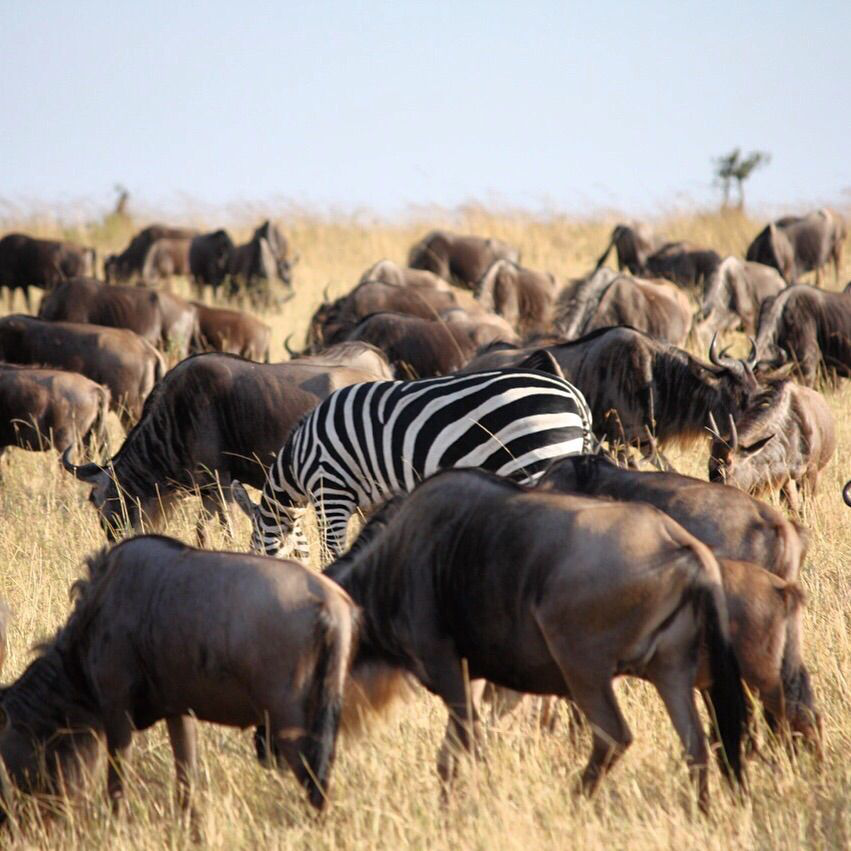
\includegraphics[width=.5\linewidth]{./images/figures/zibra-anomaly.png}\hfill
			  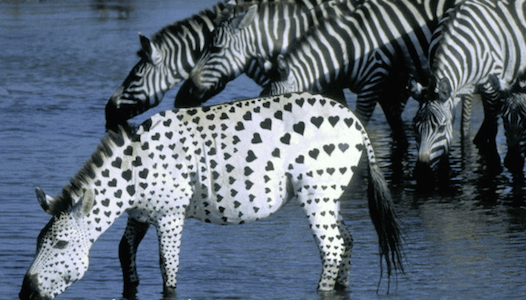
\includegraphics[width=.5\linewidth]{./images/figures/zibra-novel.png}
		  \end{subfigure}\par\medskip		  
		  \caption{مثالی از تفاوت دادگان ناهنجار و نوین}
		  \label{fig:novel-vs-anomaly}
	\end{figure}

در کنار ناهنجاری‌ها، دادگان دیگری نیز وجود دارند که با دادگان عادی متفاوت‌اند امّا این تفاوت به اندازی کافی زیاد نیست. به این دادگان اصطلاحا دادگان نوین\LTRfootnote{\lr{Novelties}} گفته می‌شود. دادگان نوین درواقع دادگانی هستند که در دسته دادگان عادی قرار می‌گیرند اما چون هنوز کشف نشده‌اند به نظر می‌رسد که با دادگان عادی تفاوت داشته باشند. برای مثال، اکثر ببر‌های دیده شده و شناخته شده به رنگ نارنجی و با خطوط راه راه سیاه هستند و دیدن بربر سفید برای ما تعجب آور خواهد بود. امّا همه به خوبی می‌دانیم که ببر سفید درواقع یک ببر است که فقط رنگ آن غیرعادی است و نباید آن را در دسته جدایی از حیوانات قرار داد.\\

در ادامه این فصل پس از تعریف ناهنجاری در دادگان، به بیان کاربرد‌های این بحث در حوزه‌های مختلف می‌پردازیم. سپس یک تعریف معیار که مرتبط با حوزه مورد نظر ما که همان پردازش تصویر است ارائه می‌دهیم. پس از تعریف حوزه مورد مطالعه و بررسی اهمیت موضوع، به توضیح ساختار کلی گزارش این سمینار خواهیم پرداخت.
		
	\section{مسئله تشخیص ناهنجاری}
تشخیص ناهنجاری که با عنوان تشخیص دادگان خارج از محدوده\LTRfootnote{Outlier detection} نیز شناخته می‌شود، به عملیاتی گفته می‌شود که طی آن به آشکارسازی نمونه‌هایی از مجموعه دادگان می‌پردازد که تفاوت زیادی با اکثریت دادگان موجود دارد. در واقع، اینجا تفاوت به معنی متفاوت بودن مشخصات و ویژگی‌های این نمونه‌ها با الگوی معمول موجود در مجموعه دادگان است. این مسئله یک موضوع فعال تحقیق در دهه‌های اخیر بوده که تقریبان از سال ۱۹۶۰ میلادی تا کنون مورد مطالعه قرار گرفته است~\cite{Grubbs1969ProceduresFD}. کاربردهای تشخیص ناهنجاری بسیار وسیع است و در حوزه‌های گوناگونی مورد استفاده قرار می‌گیرد.\\

ناهنجاری‌ها انواع مختلفی دارند که بسته به کاربرد و مفاهیم مختلف تعریف می‌شوند. به طور کلی می‌توان برای ناهنجاری‌ها سه نوع مختلف درنظر گرفت که عبارت اند از ناهنجاری نقطه‌ای\LTRfootnote{Point anomaly}،‌ ناهنجاری مفهومی‌\LTRfootnote{contextual anomalies}،‌ ناهنجاری مجموعه‌ای\LTRfootnote{collective anomalies}. اکثرکارهای انجام شده در متون علمی در مورد ناهنجاری نقطه‌ای بحث شده است. در این گونه ناهنجاری دادگان به صورت نقاطی در فضا درنظر گرفته می‌شوند و دادگان ناهنجار، نقاطی در فضای مورد نظر هستند که با دیگر دادگان فاصله دارند و رفتاری تصادفی از خود نشان می‌دهند که اغلب تفسیر خاصی ندارند. برا مثال مبلغ بسیار بالای تراکنش در یک رستوران  یک تراکنش غیر عادی به حساب می‌آید که با در نظر گرفتن آن در فضای بازنمایی دادگان این نقطه شباهتی به دیگر دادگان نخواهد داشت. دسته دوم ناهنجاری‌های مفهومی هستند که در این دسته مفهموم داده در یک مکان‌ و یا زمان‌ مختلف می‌تواند به صورت ناهنجاری درنظر گرفته شود. برای مثال عبور وسیله نقلیه در خیابان یک امر طبیعی است اما عبود وسایل نقلیه در مسیر عابرین پیاده یک پدیده غیرعادی است. نوع سوم ناهنجاری‌ها که اصطلاحا ناهنجاری مجموعه‌ای گفته می‌شود،‌مفهوم ناهنجاری از در یک سلسله از رویدادها دنبال می‌کند در حالی که هر رویداد یک داده کاملا عادی است. برای مثال در دنباله تراکنش‌های یک کارت اعتبار وجود چندین تراکنش یکسان با فاصل زمانی بسیار کم مشکوک است.

\begin{figure}[!hp]
	\begin{center}
		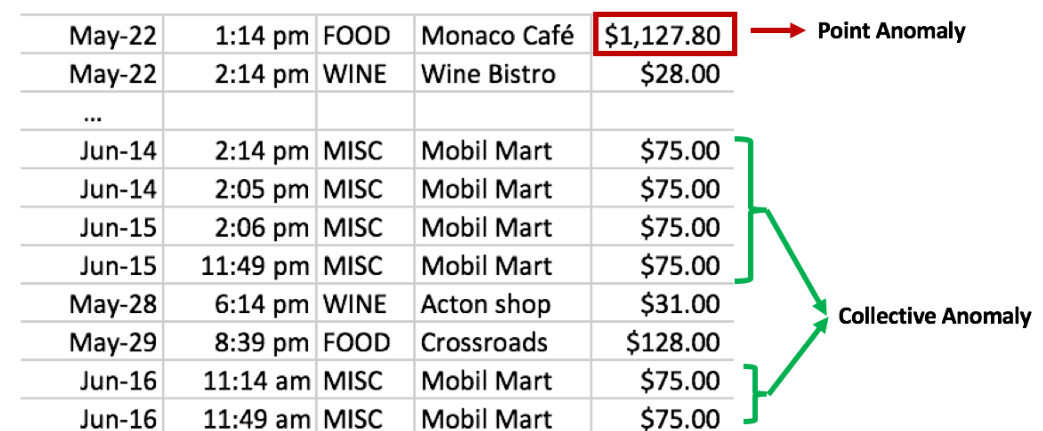
\includegraphics[width=\linewidth]{./images/figures/credit-card.png}

		\caption{
		ناهنجاری نقطه‌ای و دنباله‌ای
		\cite{G.Chalapathy}
		}		
		\label{fig:anomaly-example-1}
		\centering
	\end{center}
\end{figure}



\begin{figure}[hp]
	\begin{center}
		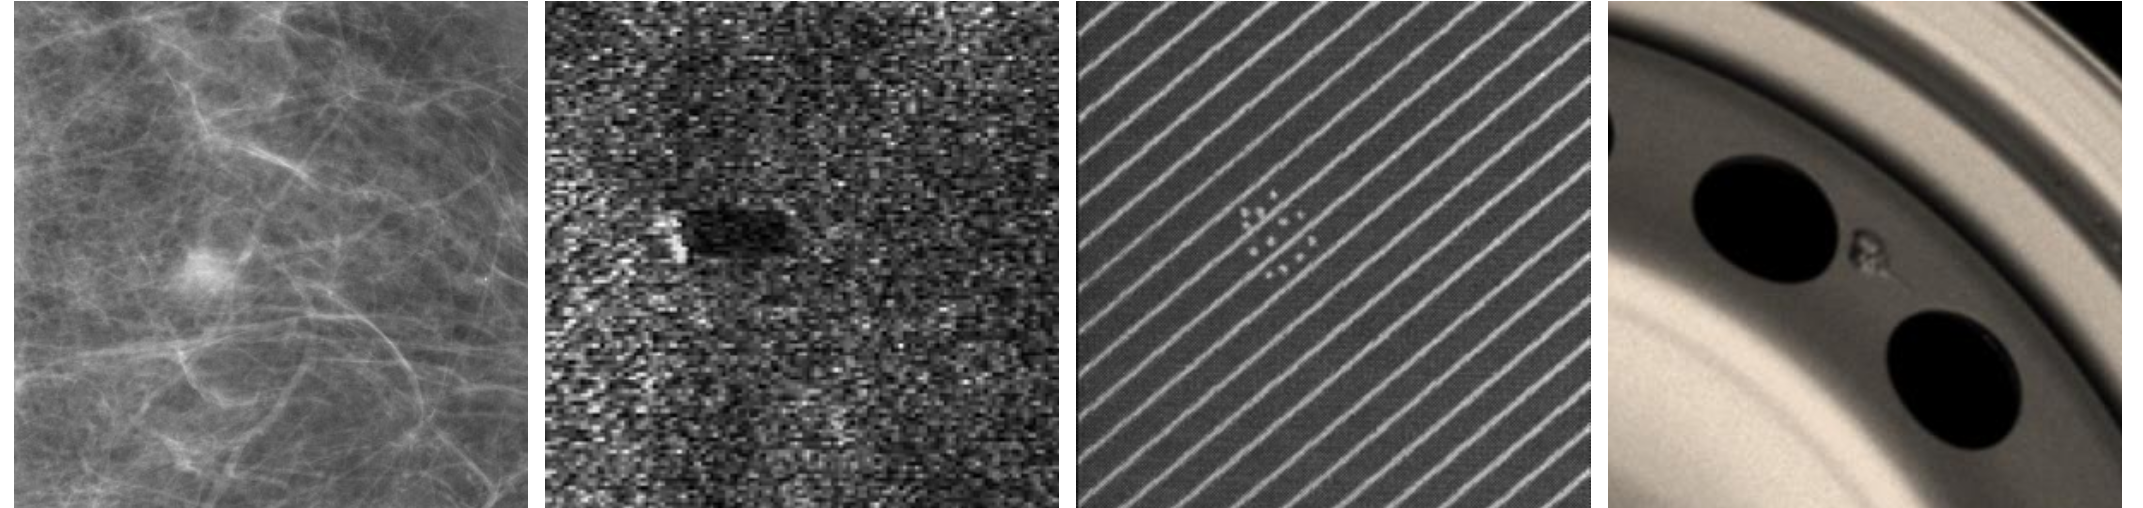
\includegraphics[width=\linewidth]{./images/figures/image-anomaly-examples-1.png}
		\caption*{به ترتیب از سمت چپ، توده سرطان سینه، مین زیر‌دریایی، نقص رنگ‌آمیزی کاشی تولید شده در کارخانه،نمونه نقص موجود در چرخ خودرو.}
		\caption{
		مثال‌هایی از ناهنجاری در تصاویر
		\cite{T.Ehret}
		}		
		\label{fig:anomaly-example-1}
		\centering
	\end{center}
\end{figure}

\section{ساختار کلی روش‌های تشخیص ناهنجاری}
	اگر بخواهیم روش‌های تشخیص ناهنجاری را به صورت عمومی توصیف کنیم، می‌توانیم بگوییم که این روش‌ها از سه بخش اصلی تشکیل شده‌اند. بخش اوّل یادگیری بازنمایی داد‌ه‌ها\LTRfootnote{Data representation} است. در این مرحله نگاشتی از دادگان ورودی به فضایی معیین آموخته می‌شود. این نگاشت را می‌توان به صورت تابعی مانند زیر تعریف کرد.
\begin{equation}
f(.;\theta): x \rightarrow y
\end{equation}
	
در بخش دوّم به تعریف یک معیار سنجش پرداخته می‌شود که برای ارزیابی خروجی مرحله قبل استفاده می‌شود. این معیار با دریافت خروجی مرحله اوّل یک امتیاز برای سنجش میزان تعلق داده ورودی به دسته ناهنجار اختصاص می‌دهد که به آن امتیاز ناهنجاری\LTRfootnote{Anomaly score} گوییم.
\begin{equation}
d(f(x);\eta): f(x) \rightarrow d \  ,\  d \in \mathbb{R}
\end{equation}

در آخر نیز با درنظر گرفتن یک مقدار آستانه $\delta$، به تصمیم‌گیری در مورد داده ورودی با توجه به امتیاز اختصاص داده شده در مرحله دوّم پرداخته می‌شود.

$$
\left\{
	\begin{array}{ll}
		anomaly  & d \geq \delta \\
		not\ anomaly & d < \delta
	\end{array}
\right.
$$

با توجه به این تعریف، رویکرد‌های موجود می‌توانند انواع زیر را داشته باشند:
\begin{enumerate}
	\item {غیر پارامتری: نیازی به یادگیری $\theta$ و $\eta$ و $\delta$ نیست.}
	\item{یک مرحله‌ای: تنها یکی از مجموعه پارامترهای موجود $\theta$ یا  $\eta$ یاد‌گرفته می‌شوند.}
	\item{دو مرحله‌ای:‌ هر دو مجموعه پارامتر $\theta$ و $\eta$ به صورت مستقل و جداگانه یاد‌گرفته می‌شوند.}
	\item{ادغامی\LTRfootnote{Integrated}: هر دو مجموعه پارامتر $\theta$ و $\eta$ باهم یادگرفته می‌شوند. }
\end{enumerate}

درصورت عدم وجود برچسب‌های دادگان موجود، ناچار به استفاده از روش بدون ناظر هستیم که در آن از هیچ گونه اطلاعاتی در مورد ماهیت دادگان استفاده نمی‌شود. در  این گونه مواقع معمولا $\delta$ از پیش تعریف شده است و یا همراه با  $\eta$ یادگرفته می‌شود. در حالتی که تنها بخشی از دادگان برچسب خورده باشند و باقی برچسب نخورده، می‌توانیم از رویکرد یادگیری با نظارت ضعیف استفاده کرد. در این مورد نیز مقدار آستانه می‌تواند با استفاده از تنظیم دقیق مدل بدست آید.
	
	\section{ساختار گزارش}
در فصل اوّل این سمینار به معرفی حوزه سمینار و تعریف مسئله پرداخته شد و در فصل دوّم به تعریف مفاهیم و اصطلاحات استفاده شده در این حوزه خواهیم پرداخت. فصل سوّم نیز در رابطه با بررسی کار‌های مرتبط با این سمینار و معرفی و بررسی جزئی از روش‌ها و مقالات موجود چاپ شده در سال‌های اخیر خواهد پرداخت. در ابتدای فصل سوّم پس از معرفی کار‌های مرتبط یک دسته‌بندی از روش‌های موجود ارائه می‌گردد و در ادامه، ترتیب معرفی و بررسی روش‌های موجود بر طبق این دسته‌بندی خواهد بود. در نهایت یک جمع بندی و نتیجه گیری کلی از روش‌های موجود در هر دسته انجام می‌دهیم و پیشنهاداتمان را در رابطه با استفاده از این روش‌ها بسته به کاربرد مورد نظر ارائه می‌کنیم. در فصل آخر گزارش پیشنهادات خود را درباره کار‌های آینده این حوزه ارائه کرده و در نهایت پیشنهاد انجام پروژه کارشناسی ارشد را که در راستای همین سمینار است معرفی می‌کنیم.
	%------------Chapter 2--------------
	\chapter{مروری بر روش‌های سنتی}
	اگر به‌یاد داشته باشید، در ابتدای فصل یک به این نکته اشاره شد که مسئله تشخیص ناهنجاری، یک موضوع فعال تحقیق در چند دهه اخیر است که یکی از مقالات معتبر چاپ شده آن مربوط به دهه ۱۹۶۰ میلادی می‌شود. از این رو، در طی این مدت بسیاری از روش‌ها برای یافتن دادگان خارج از محدوده معرفی و توسعه داده شده‌اند که از یادگیری عمیق استفاده نمی‌کنند. این روش‌ها به صورت عمده دادگان را مجموعه‌ای از نقاط در یک فضای چند بعدی فرض می‌کنند و تلاش آنها برای این است که نقاط خارج از محدوده را در این فضا با توجه به ویژگی‌ها و مشخصات دیگر نقاط آشکار کنند. عمدتاً این اینگونه روش‌ها را می‌توان از نقطه‌نظر ایده اصلی به سه دسته کلی استفاده از رده‌بندی، معیار فاصله و مدل‌های آماری تقسیم کرد\footnote{ر.ک جدول~\ref{table:traditional-category}}. در ادامه به مرور کلی این روش‌ها خواهیم پرداخت. با توجه به اینکه تمرکز ما بر بررسی کامل این روش‌ها نیست پیشنهاد می‌شود برای آشنایی بیشتر با این‌گونه روش‌ها به مقاله چاندولا و همکاران مراجعه کنید~\cite{V.Chandola}.
	
\begin{center}
\begin{table}[!h]
\begin{tabular}{ |p{4cm}|p{4cm}|p{4cm}|p{4cm}| } 
\hline
\multicolumn{4}{|c|}{دسته‌بندی روش‌های سنتی در تشخیص ناهنجاری}  \\
\hline

مبتنی بر ‌ & خلاصه ایده& انواع & روش‌های شناخته شده \\
\hline
رده‌بندی & یادگیری یک مرز تفکیک میان دادگان عادی و ناهنجار & یک کلاسه & \latin{One-class SVM} \latin{SVDD} \\
\cline{3-4}
& & چند کلاسه & - \\

\hline
معیار فاصله & اقدام به تعریف یک معیار فاصله می‌کند تا دادگان عادی را از دادگان ناهنجار جدا کند &  فاصله تا نزدیک ترین همسایه &  \latin{LOC}\LTRfootnote{Local Outlier Factor}  \latin{COF} \\
\cline{3-4}
&&خوشه بندی و سنجش فاصله تا نزدیک ترین خوشه& \latin{K-means} \latin{CBLOF} \\

\cline{3-4}
&&استفاده از تصویر سازی نقاط در فضایی با ابعاد کمتر& \latin{PCA} \latin{Isolation Forest} \\

\hline 
مدل آماری & دادگان عادی در نواحی پر احتمال مدل آماری قرار می‌گیرند & روش‌های پارامتری  & \latin{Gausian Mixture Model} \\
\cline{3-4}
&&روش‌های غیر پارامتری ‌& \latin{Kernel destiny estimator} \\
\hline

\end{tabular}
\caption{دسته‌بندی روش‌های سنتی}
\label{table:traditional-category}
\end{table}
\end{center}

\section{روش‌های مبتنی بر رده‌بندی}
همانطور که در ابتدای این بخش گفته شد، یکی از ایده‌های کلی در روش‌های مورد استفاده برای تشخیص ناهنجاری استفاده از ایده رده‌بندی است. در اینگونه روش‌ها تلاش می‌شود یک مرز تفکیک میان دادگان عادی و دادگان ناهنجار رسم شود. اگر چنین مرزی وجود داشته باشد، می‌توانیم با استفاده از الگوریتم‌های رده‌بند موجود اقدام به یافتن این مرز کرد و سپس با استفاده از مدل آموزش دیده اقدام به آشکارسازی داده‌های ناهنجار کرد. همانطور که مشخص است در این گونه روش‌ها تنها یک دسته برای دادگان تعریف می‌شود که آن دسته دادگان عادی است. دیگر دادگانی که در این دسته قرار نمی‌گیرند به عنوان دادگان عادی در نظر گرفته می‌شوند. البته استفاده از رویکرد رده‌بندی چند کلاسه نیز در صورت وجود برچسب برای تمامی دادگان امکان پذیر است امّا استفاده از این روش کمتر مرسوم است. یکی از معروف ترین روش‌های مورد استفاده دسته بند بردار پشتیبان یک کلاسه\LTRfootnote{One-class SVM} است.

در ماشین بردار پشتیبان ما به دنبال یافتن یک ابر صفحه جدا کننده میان دو دسته داده موجود هستیم. در الگوریتم بردار پشتیبان یک کلاسه ما درواقع به دنبال یافتن صفحه ای هستیم که دادگان معمول در یک طرف این صفحه قرار بگیرند. در این روش تلاش می‌شود صفحه مورد نظر تا حد امکان به نقاد داده نزدیک باشند. پس از رسم این صفحه، دادگانی که به مبدا مختصات نزدیک تر هستند در دسته ناهنجاری‌ها قرار می‌گیرند \cite{10.5555/3009657.3009740}.

در اینجا تابع نگاشتی که باید یاد کرفته شود همان تابع کرنل در ماشین بردار پشتیبان است و تابع امتیاز ناهنجاری نیز به صورت اندازه فاصله از مبدا مختصات تعریف می‌شود. شکل~\ref{fig:one-class-svm} این روش را به تصویر کشیده است. توجه داشته باشید که در اینجا تنها یک دسته برای رده‌بندی تعریف می‌شود که آن دسته دادگان عادی است، پس نیازی به وجود برچسب برای تمامی دادگان نیست و رویکرد ما در اینجا به صورت کاملا بدون ناظر خواهد بود.
\begin{figure}[!h]
	\begin{center}
		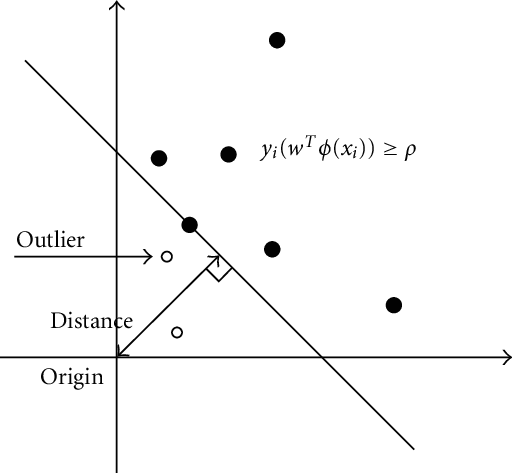
\includegraphics[width=0.5\linewidth]{./images/figures/one-class-svm.png}
	\end{center}
	\caption{ماشین بردار پشتیبان یک کلاسه}
	\label{fig:one-class-svm}
	\centering
\end{figure}


نمونه دیگری از روش‌های مورد استفاده برای آشکارسازی ناهنجاری که از رویکرد رده‌بندی استفاده می‌کند، بردار پتیبان توصیفگر داده‌\LTRfootnote{Support Vector Data Description (SVDD)} است. در این روش سعی می‌شود کره‌ای با کوچک ترین اندازه ممکن حول دادگان موجور رسم شود. پس از رسم این کره، دادگانی که در خارج از آن قرار می‌گیرند به عنوان داده ناهنجار شناخته خواهند شد~\cite{pmlr-v80-ruff18a} .
\begin{figure}[!h]
	\begin{center}
		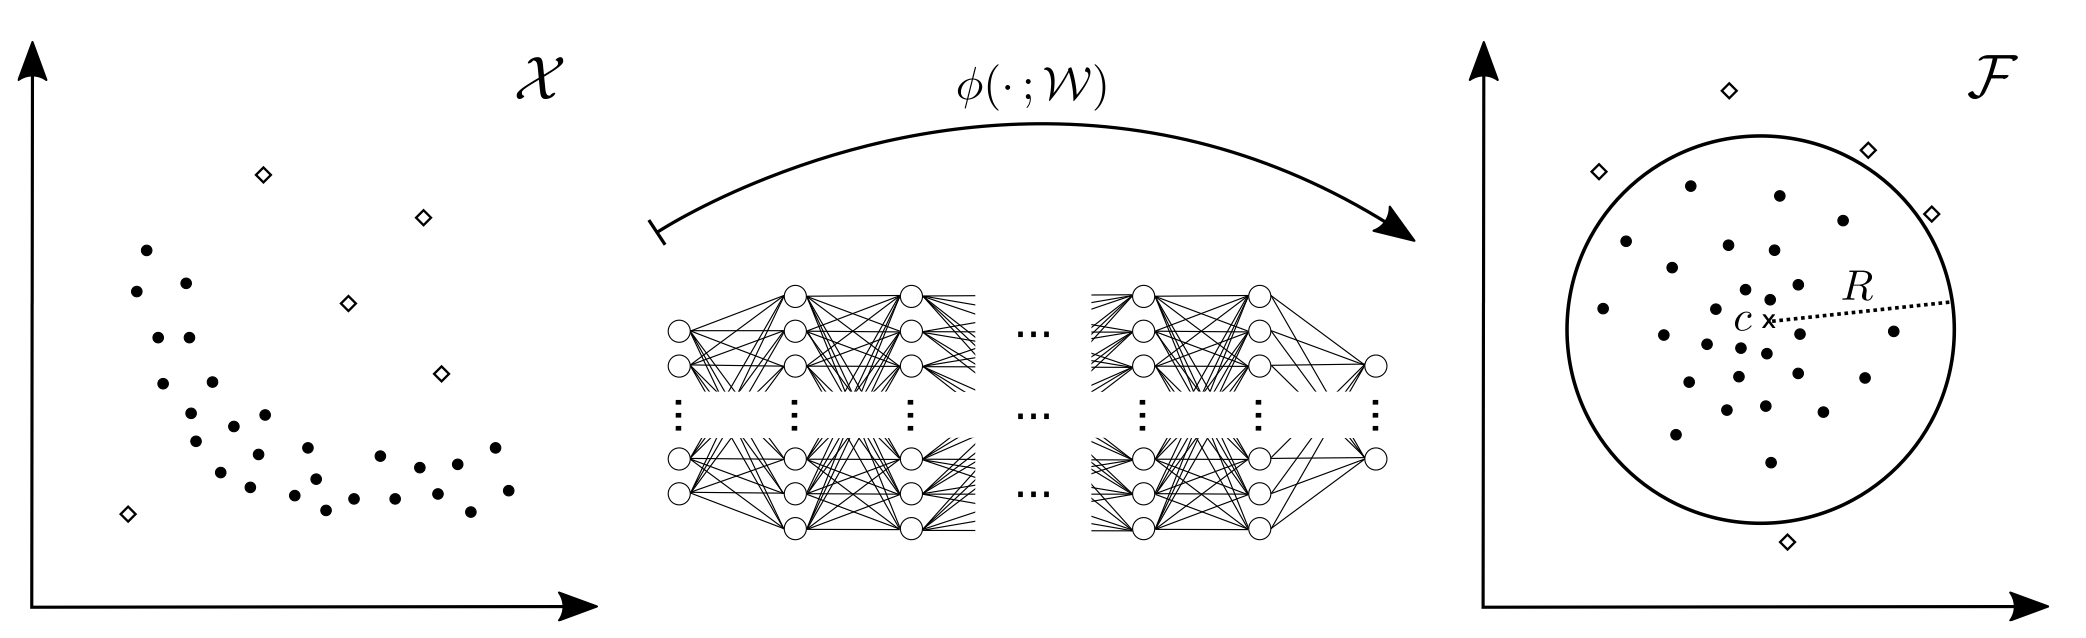
\includegraphics[width=\linewidth]{./images/figures/deep-svdd.png}
	\end{center}
	\caption{بردار پشتیبان توصیفگر داده عمیق~\cite{pmlr-v80-ruff18a}}
	\label{fig:deep-svdd}
	\centering
\end{figure}

ازجمله مزیت‌های این رویکرد،‌آموزش سریع، و دقت بهتر آن در مواقعی است که دادگان برچسب خورده در اختیار هستند. و از معایب این روش در هنگام استفاده از رده‌بندی چند کلاسه می‌توان به نیاز برای چندین دسته داده عادی یاد کرد. همچنین این این رویکرد‌ها نیاز به تعیین ابر پارامتر برای مدل یادگیری دارند.

\section{روش‌های مبتنی بر معیار فاصله}
اگر به دادگان موجود را به صورت نقاطی بازنمایی شده بر روی صفحه مختصات نگاه کنیم،‌ می‌توانیم از معیار فاصله نقاط از یکدیگر به تصمیم‌گیری در مورد دادگان بپردازیم. در اینگونه رویکرد‌ها معمولا اقدام به تعریف یک معیار فاصله می‌کنند تا دادگان عادی را از دادگان ناهنجار جدا کنند. یک نمونه روش معروف که در این دسته می‌گنجد روش معروف عامل پرت محلی\LTRfootnote{Local Outlier Factor} است. در این روش میانگین فاصله هر نقطه از همسایگان محلی محاسبه شده و اگر این میانگین از یک مقدار آستانه بیشتر باشد،‌داده به عنوان داده ناهنجار شناخته می‌شود. برای سادگی کار، میانگین فاصله نقطه تا تمام همسایگان را بر میانگین فاصله میان همسایگان نقطه محاسبه شده و مقدار آستان برابر با عدد یک درنظر گرفته می‌شود~\cite{10.1145/342009.335388}. در استفاده از این روش نیز نیازی به وجود برچسب دادگان نیست همچنین این روش پارامتری برای یادگیری ندارد و در دسته روش‌های بدون پارامتر نیز قرار می‌گیرد. در واقع این گونه روش‌ها معمولا به صورت بدون ناظر هستند.


	\begin{figure}[!h]
	\begin{center}
		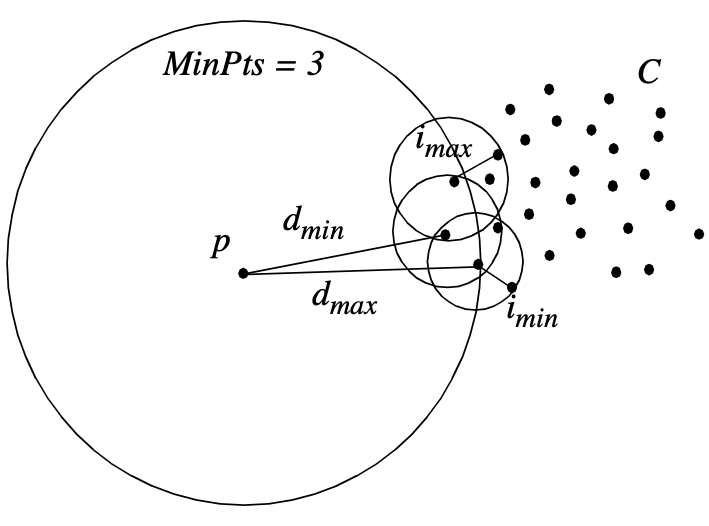
\includegraphics[width=0.5\linewidth]{./images/figures/lof.png}
	\end{center}
	\caption{نمایش کلی روش عامل پرت محلی~\cite{10.1145/342009.335388}}
	\label{fig:lof}
	\centering
\end{figure}



\section{روش‌های مبتنی بر مدل آماری}
ایده اصلی در این دسته از رویکرد‌ها بدین صورت است که، دادگان عادی همواره احتمال رخدادن بالایی دارند، در نتیجه در نواحی از مدل مدل آماری قرار می‌گیرند که احتمال وقوع آنها بیشتر است. برای مثال در روش مدل خطی پویا\LTRfootnote{Dynamic liner model} ابتدا دادگان را از فضای ورودی به یک فضای از پیش تعیین شده نگاشت می‌کنیم. سپس با استفاده از مدل بدست آمده سعی در پیشبینی مقدار ورودی با توجه به دیگر دادگان موجود می‌کنیم. در اینجا امتیاز ناهنجاری میزان تفاوت مقدار پیشبینی شده و مقدار حقیقی داده است. اگر مقدار اختلاف از یک مقدار آستانه از پیش تعیین شده، که با استفاده از آزمایش با دادگان برچسب خورده بدست آمده، بیشتر باشد، به دسته دادگان ناهنجار تعلق می‌گیرد.


	\chapter{روش‌های مبتنی بر یادگیری عمیق}
	در این فصل‌ ابتدا به معرفی مدل‌های پایه‌ای یادگیری عمیق خواهیم پرداخت که در تشخیص ناهنجاری مورد استفاده قرار می‌گیرند. ینگونه مدل‌ها، پایه و اساس خیلی از روش‌های ارائه شده هستند و آشنایی با آنها به درک بهتر مطلب کمک بسیار زیادی خواهد کرد. پس از معرفی ساختار مورد بحث نمونه‌هایی از کار‌های انجام شده که از آن استفاده می‌‎کنند را به اختصار معرفی خواهیم کرد. جدول~\ref{table:deep-structures} لیستی از تمام روش‌های مورد بحث در این بخش را جمع آوری کرده است.

	
\begin{table}[!h]
	\begin{center}
			\begin{tabular}{ |c|c|c| } 
				\hline
				\multicolumn{3}{|c|}{مدل‌های پایه‌ مورد استفاده در روش‌های عمیق برای تشخیص ناهنجاری}  \\
				\hline
				
				نام مدل ‌ & مقاله مرجع & مزیت استفاده \\
				\hline
				\latin{AE} & & \\
				\hline
				\latin{VAE} & & \\
				\hline
				\latin{SAE} & & \\
				\hline
				\latin{ِDCAE} & & \\
				\hline					
				\latin{DTS} & & \\
				\hline
				\latin{GAN} & & \\
				\hline	
			
			\end{tabular}
			\caption{الگوریتم‌های عمیق مورد استفاده در تشخیص ناهنجاری}
			\label{table:deep-structures}
		\end{center}
\end{table}

	\section{مدل پرسپترون چند لایه‌ای}
مدل پرسپترون چند لایه‌ای\LTRfootnote{Multilayer Perceptron} یکی از ابتدایی ترین و مهم‌ترین مدل‌هایی است که می‌توان آنرا نقطه شروعی بر تمام روش‌های عمیق موجود در حال حاضر دانست. این مدل درواقع شبکه‌ای از نورون‌های عصبی مصنوعی\LTRfootnote{Perceptron} است که لایه‌های آن صورت کاملا متصل با یکدیگر ارتباط دارند. این شبک دارای حداقل سه لایه ورودی، مخفی و خروجی است که در آن به غیر از نورون‌های لایه ورودی، باقی نورون‌ها دارای تابع فعال سازی غیر خطی هستند. این مدل برای یادگیری بازنمایی غیر خطی دادگان ورودی معرفی شده و در بسیاری از روش‌های تشخیص ناهنجاری کاربرد دارد.

\begin{figure}[!h]
	\begin{center}
		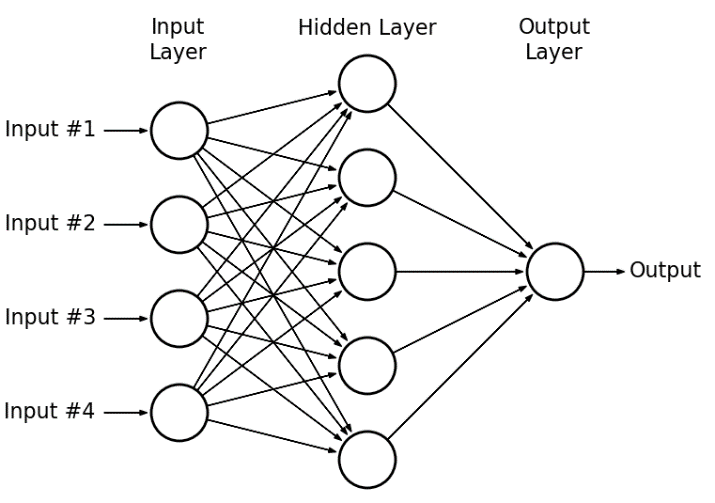
\includegraphics[width=0.5\linewidth]{./images/figures/mlp.png}
	\end{center}
	\caption{مدل پرسپترون چند لایه}
	\label{fig:mlp}
	\centering
\end{figure}

	\section{خود رمزکننده}
	خودرمز کننده‌\LTRfootnote{AutoEncoder}ها نوعی از شبکه‌های عصبی هستند که از روش پس انتشار\LTRfootnote{Backpropagation} برای یادگیری ویژگی‌های مفهومی استفاده می‌کنند. این شبکه‌ها به صورت دو مرحله‌ای اقدام به یادگیری می‌کنند که به ترتیب رمزنگاری و رمزگشایی نام دارند. در مرحله اول داده ورودی به شبکه رمز کنند داده می‌شود و رمز کننده داده ورودی را به یک فضا با ابعاد پایین نگاشت می‌کند. به این فضا به اصطلاح فضای باقی‌مانده یا فضای $z$ می‌گویند. در مرحله دوم، بازنمایی بدست آمده وارد شبکه رمز کنند شده تا داده از فضای باقی مانده دوباره به فضای ورودی باز گردانده شود. آنچه که انتظار می‌رود آن است که خروجی مدل با آنچه در ورودی به مدل داده شده بسیار شبیه باشند. در این صورت قسمت رمز کنند تواسنسته بازنمایی خوبی از داده را در فضای باقی مانده ایجاد کند~\cite{BHUVANESHWARI2021131}.
\begin{figure}[!h]
	\begin{center}
		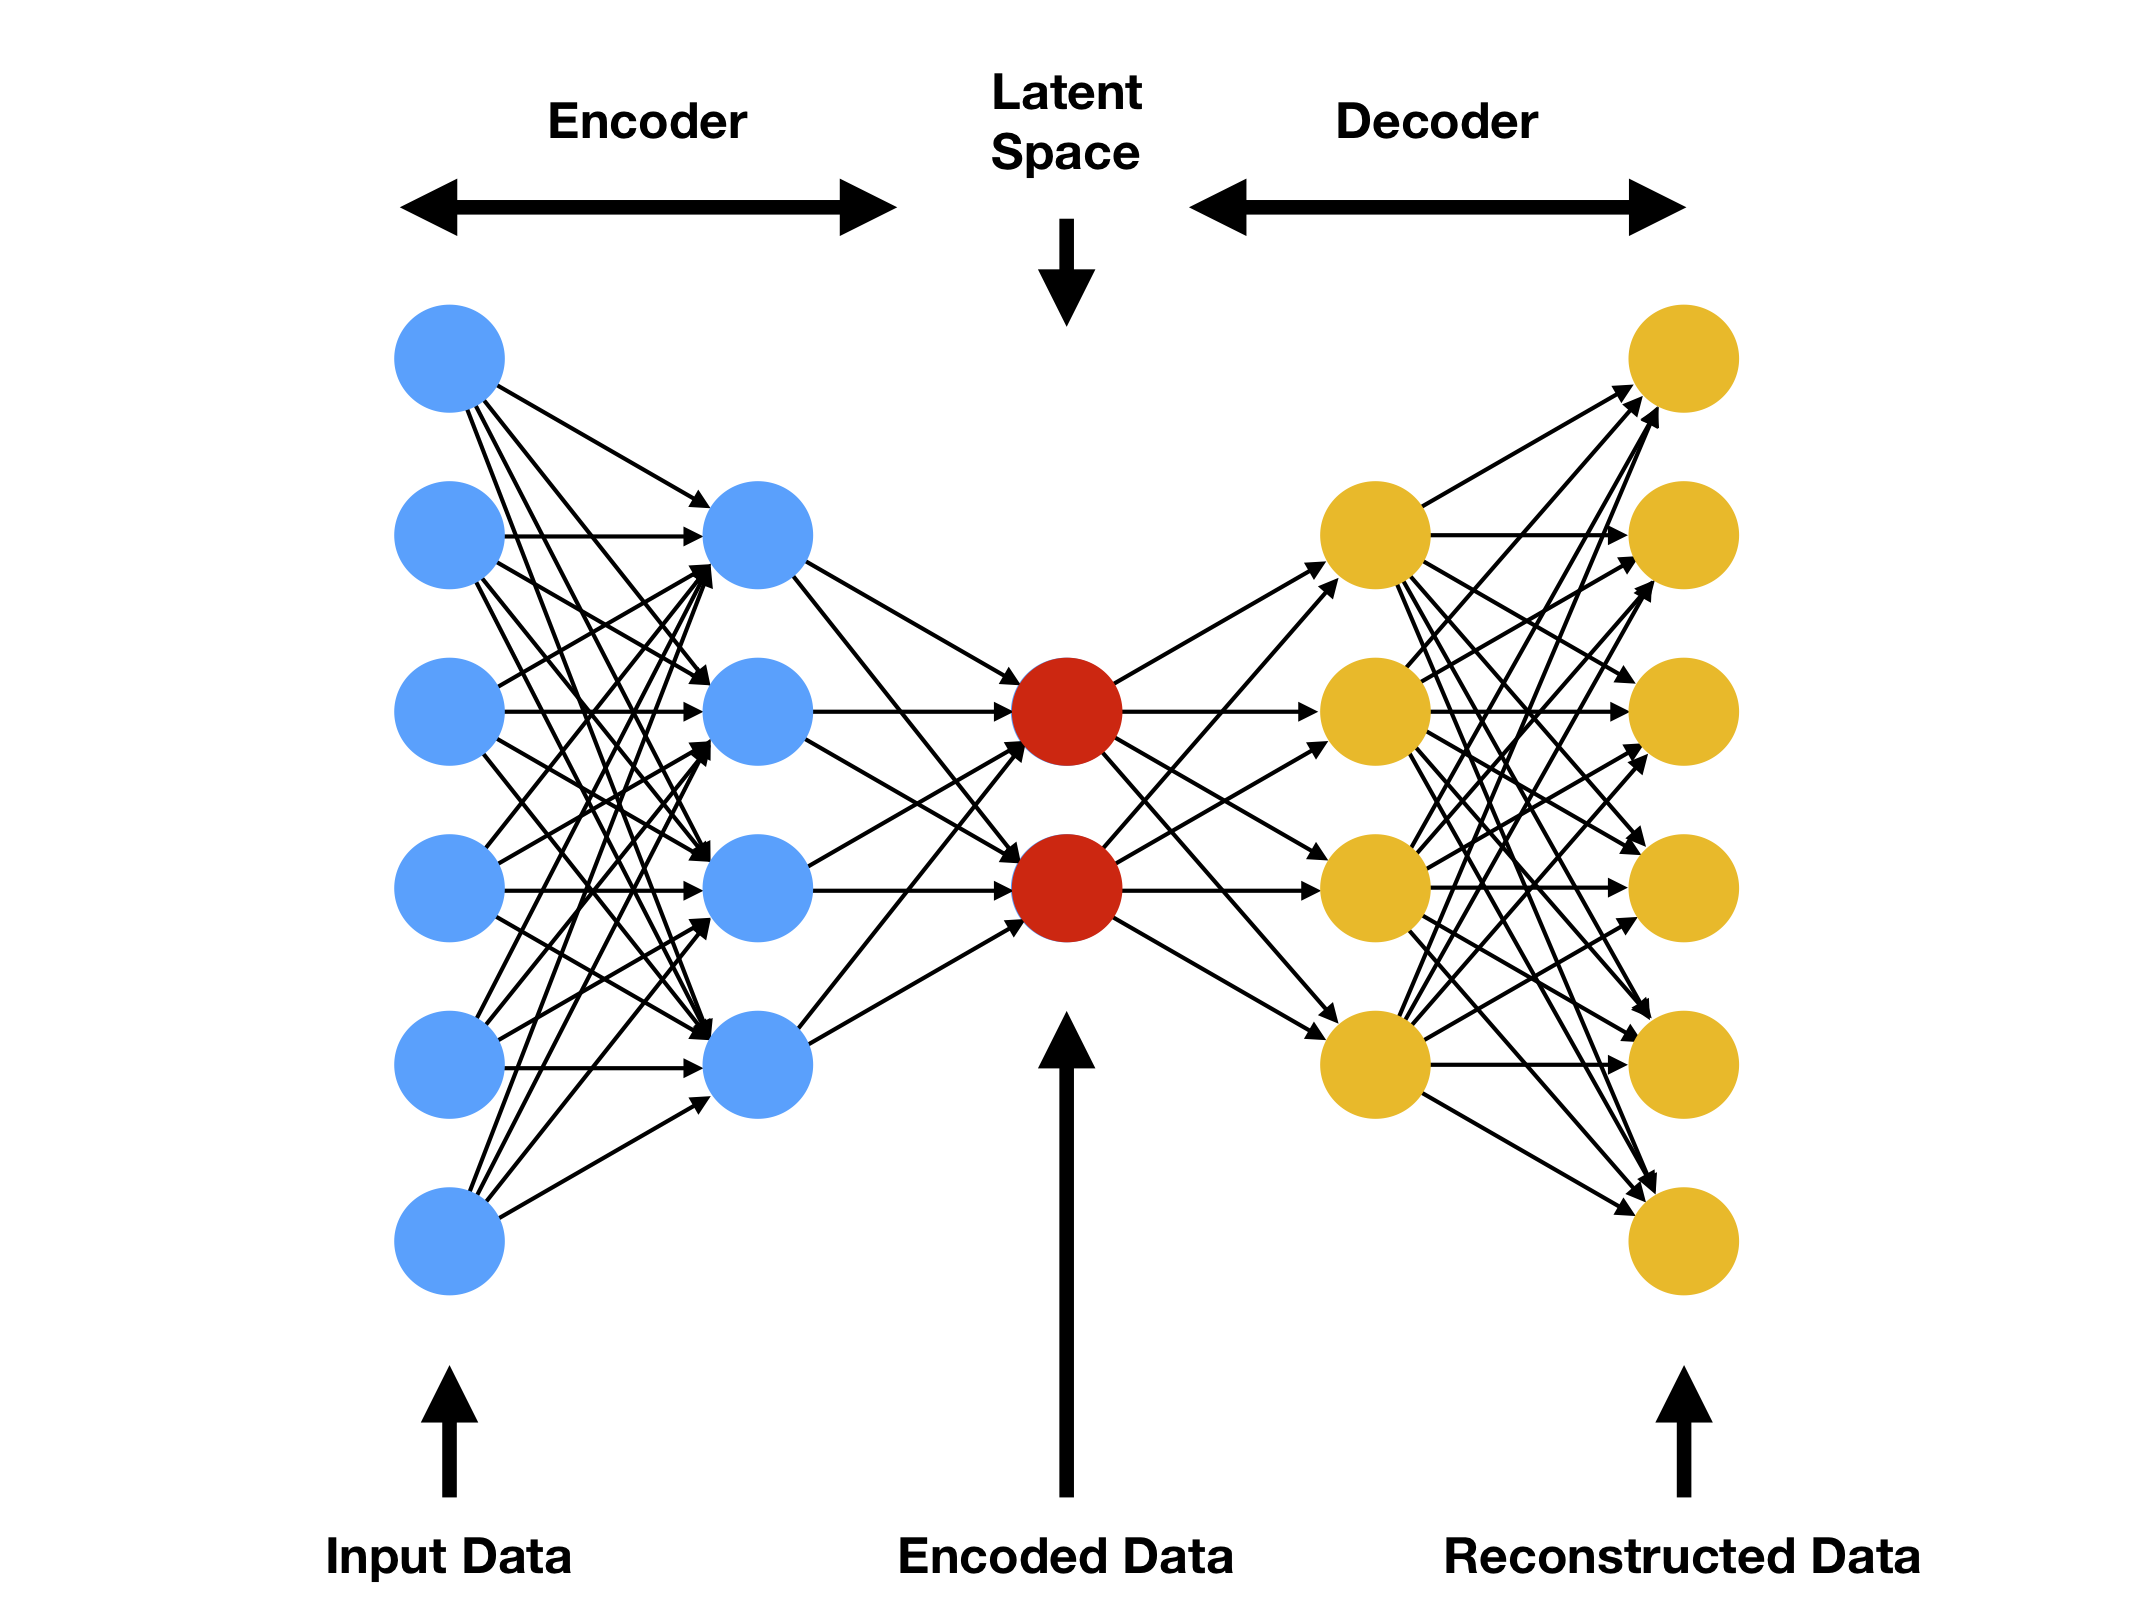
\includegraphics[width=0.6\linewidth]{./images/figures/ae.png}
	\end{center}
	\caption{مدل خود رمز کننده}
	\label{fig:ae}
	\centering
\end{figure}

اگر بخواهیم کارکرد مدل شکل~\ref{fig:ae} را با فرمول ریاضی توصیف کنیم، با در نظر داده $X$ به عنوان ورودی مدل، رمز کنند با گرفتن این ورودی، آن را به فضای باقی مانده و به نقطه $z$ نگاشت می‌کند. اگر تابع رمز کننده را $f$ بنامیم معادله مرحله اول به صورت زیر خواهد بود.
\begin{equation}
f(X, \theta_1): X \rightarrow z
\end{equation}
که در اینجا ابعاد فضای $z$ از ابعاد فضای ورودی $X$ کمتر است. این بدان معنی است که در اینجا عمل کاهش ابعاد ورودی صورت گرفته است. اگر رمزگشا را مانند تابعی درنظر بگیریم و آن‌را $g$ بنامیم، این تابع با دریافت ورودی $z$، اقدام به بازسازی داده ورودی می‌کند.
\begin{equation}
	g(z, \theta_2): z \rightarrow X
\end{equation}

در کاربردهای تشخیص ناهنجاری معمولا در هنگام استفاه از این معماری، سعی می‌شود از تابع خطای مقایسه ورودی و خروجی مدل برای آموزش مدل استفاده کنند و در فرایند آموزش تنها از دادگان عادی استفاده شود. ایده اصلی در این گونه روش‌ها این است که با توجه به اینکه مدل تنها با دادگان عادی آموزش دیده است، دادگانی که توسط این مدل نتوانند به خوبی بازسازی شوند دارای ناهنجاری بوده‌اند. در واقع در اینجا تابع خطا که همان تابع امتیاز ناهنجاری است به صورت زیر تعریف می‌شود.
\begin{equation}
	L(X, g(f(x))) = d
\end{equation}

پس از آموزش مدل مقدار آستانه $\delta$ برای بدست آوردن بهترین نتیجه با آزمون و خطا و یا روش‌های دیگر مانند استفاده از نمودار حساسیت و دقت تعیین می‌شود. \\

خودرمز کننده‌ها باید به تغییرات دادگان ورودی حساس باشند تا بتوانند با دقت مطلوب داده رمز شده را بازسازی کنند. همچنین این حساسیت نباید به اندازه‌ای باشد که باعث بشود مدل بجای یادگیری عملکرد مناسب، به حفظ کردن دادگان ورودی بپردازد و دچار بیش‌برازش بشود. برای دستیابی به چنین توازنی، انواع مختلفی از خودرمز کننده‌ها معرفی شده‌اند که با افزودن یک مقدار تنظیم کننده\LTRfootnote{Rgulizer} به تابع خطای اصلی معرفی شده، بدست می‌آیند.
\begin{equation}
	L(X, g(f(X))) + regulizer
\end{equation}

\subsection{خود رمز کننده خلوت}
خود رمز کننده خلوت\LTRfootnote{Sparse AutoEncoder (SAE)} یکی از انواع خودرمز کننده ها است. ایده اصلی این گونه رمز کننده‌ها این است که نورون‌ها لایه مخفی اگر تعدادشان کمتر از تعداد نورون‌های لایه ورودی باشد شاید نتوانند به خوبی مفاهیم پیچیده را یاد بگیرند. در نتیجه پیشنهاد می‌شود در لایه مخفی تعداد نورون‌های بیشتری قرار گیرند اما از تابع فعال سازی خلوت\LTRfootnote{Sparse} استفاده کنند. برای دستیابی به چنین هدفی میتوان از دو نوع تنظیم کنند در تابع خطای مدل استفاده کرد. نوع اول استفاده از تنظیم کننده نرم یک است\LTRfootnote{L1-Rgulizer} که معادله تابع خطا به صورت زیر خواهد بود.
\begin{equation}
L(X, g(f(X))) + \lambda \sum_{i}^{n}|a^{(h)}|
\end{equation}
و نوع دوم استفاده از \lr{KL-Divergance} به عنوان تنظیم کننده است.
\begin{equation}
L(X, g(f(X))) + \sum_{j}^{n}KL(\rho || \hat{\rho}): \hat{\rho} =  \frac{1}{m}\sum_{i}[a_i^{(h)}(x)]
\end{equation}

\begin{figure}[!h]
	\begin{center}
		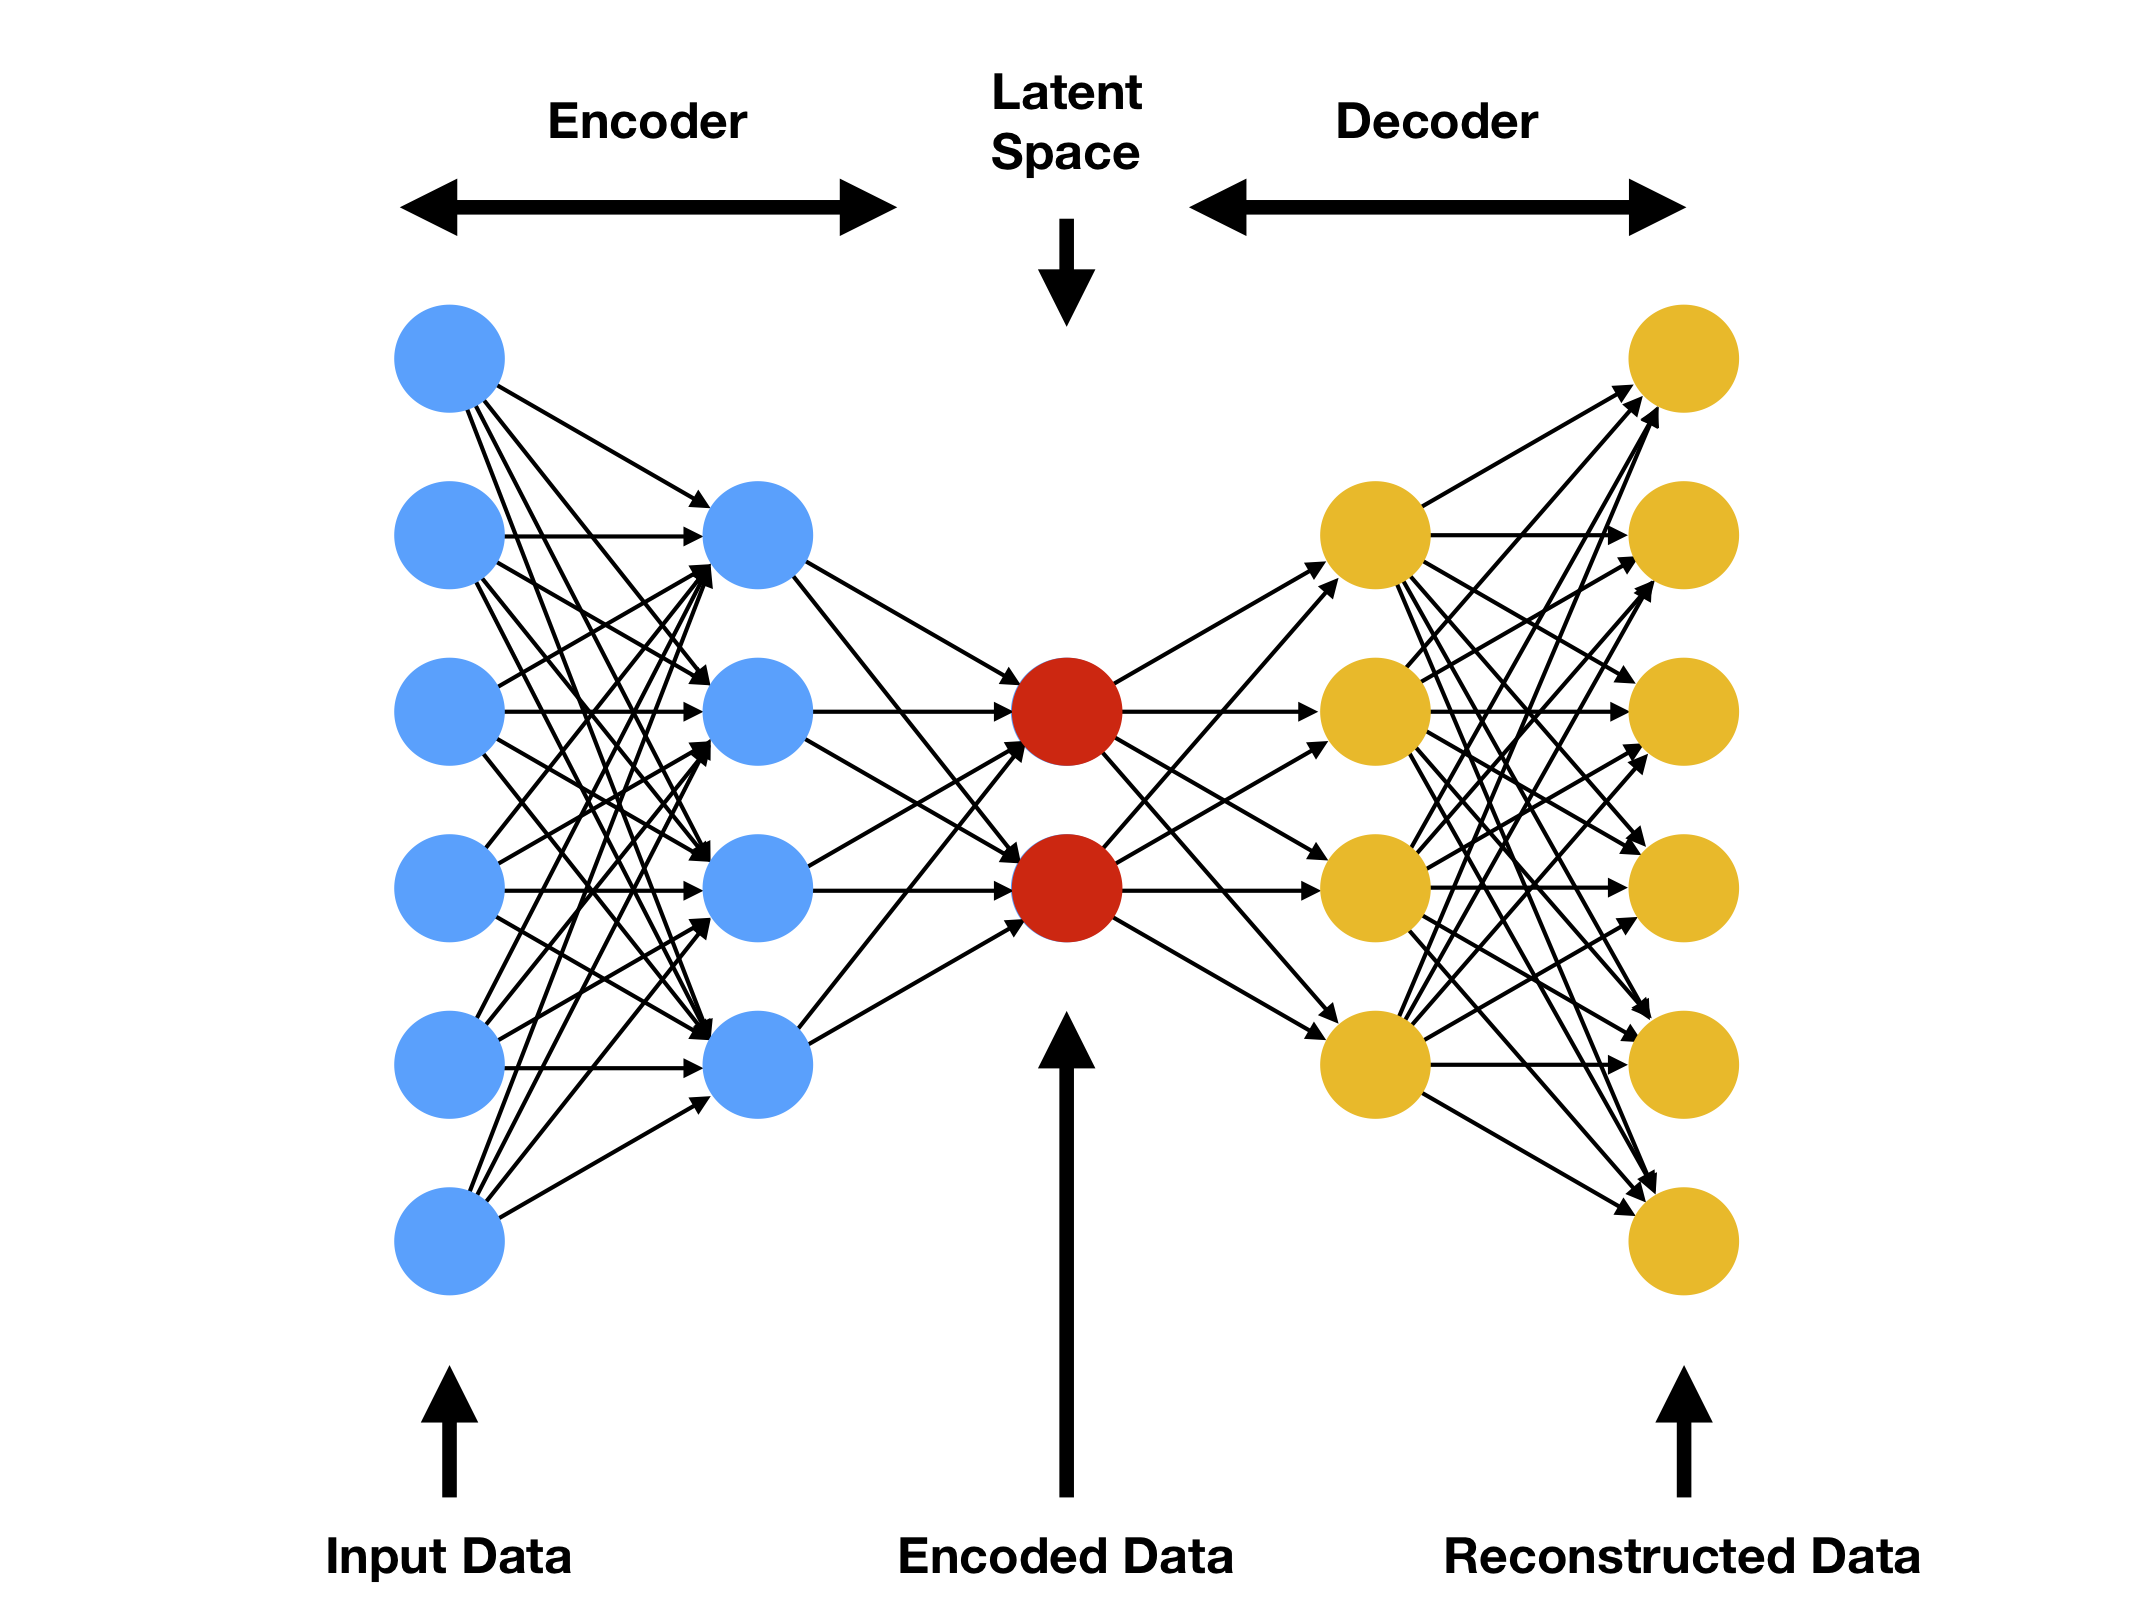
\includegraphics[width=0.6\linewidth]{./images/figures/ae.png}
	\end{center}
	\caption{مدل خود رمز کننده خلوت}
	\label{fig:ae}
	\centering
\end{figure}

	%-------------- Chapter 4--------------
	\chapter{کار‌های آینده}
	\section{نتیجه گیری}
	\section{مسائل باز و کارهای قابل انجام}
	\section{موضوع پیشنهادی برای پایان نامه}
	
	
	\newpage
%دستوری برای ظاهر شدن کلمه«مراجع» در فهرست مطالب
\addcontentsline{toc}{section}{مراجع}
%ایجاد «مراجع»
\bibliographystyle{plain-fa}
\bibliography{bibliography.bib}


%\addcontentsline{toc}{section}{نمایه}
%دستوری برای ظاهر شدن کلمه «نمایه» در فهرست مطالب(البته در صورتی که از بسته‌ای که در ابتدا گفته شد استفاده نکرده باشید)
%ایجاد «نمایه»
\printindex
\newpage
\begin{latin}
\chapter*{Abstract}
Anomaly detection is a well studied problem in varios fileds of sciance.
% صفحه آخر ترجمه انگلیسی جلد

\newpage
\thispagestyle{empty}

	\vspace*{25mm}
	\centerline{
\includegraphics[height=4cm]{./images/logos/iust.png}}

	\begin{center}
	\textbf{
Departmant of computer engineering
	}
	\\[1cm]
	\baselineskip=2cm
	{\titr
	\begin{Huge}
	Deep learning for anomaly detection\\[1cm]
	\end{Huge}}
	{\Large 
		\textbf{
			Master seminar report \\
Computer engineering - Artificial intelligence and robotics
		} \\[1cm]
	}

	{\Large { Student name:}
	\\
	{\Large  Ali Naderi Parizi}
	\\[.5cm]
	{\Large  Professor:}
	\\
	{\Large Dr.  Mohsen Soryani}
	\\[.6cm]
	}
April 2022
	\end{center}

\end{latin}
\end{document}
